\documentclass{article}
\usepackage{amsmath}
\usepackage{amssymb}
\usepackage{graphicx}
\usepackage{hyperref}
\usepackage[version=4]{mhchem}


\begin{document}
\section*{Problem}
As shown in the figure below, in \(\triangle A B C, D, E\) are the midpoints of \(A B, A C\), respectively. \(A B>A C\). Take \(F\), a point between \(D B\) such that \(D F=A E\). Draw \(F H \perp A H, A H\) is the angle bisector of \(\angle A\). Let \(H\) be the feet of the perpendicular to \(A H\) from \(F\). FH meets \(B C\) at \(M\). Show that \(B M=M C\).\\
\centering
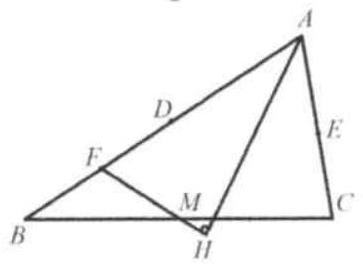
\includegraphics[width=\textwidth]{images/064(2).jpg}

\section*{Solution}
Extend \(F H\) to meet the extension of \(A C\) at \(G\).\\
Draw \(C K / / A B\). \(C K\) meets \(F G\) at \(K\).

Since \(C K / / A B, \angle B=\angle M C K\).\\
\centering
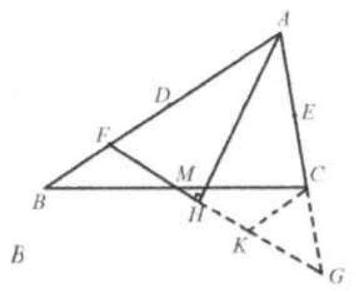
\includegraphics[width=\textwidth]{images/068.jpg}

Since \(F H \perp A H\), and \(A H\) is the angle bisector of \(\angle A\),\\
\(\angle A F H=\angle A G H, A F=A G\).\\
We also know that \(\angle B M F=\angle C M K\) (vertical angles).\\
\(A F=A G \quad \Rightarrow A D+D F=A E+E C+C G\)\\
\(\Rightarrow \quad(D F+B F)+D F=A E+A E+C G\)\\
Since \(D F=A E\), (1) becomes: \(A E+B F+A E=A E+A E+C G \quad \Rightarrow B F=C G\).\\
Since \(C K / / A B, \angle A F H=\angle A G H=\angle G K C\).\\
Thus \(C G=C K=B F\).\\
Therefore, \(\triangle B F M \cong \triangle C K M\) and \(B M=M C\).

\end{document}
